\section{Frontend}

The evaluation of the Elephant browser and the NetInfService applications tries to answer the following core questions:

\begin{enumerate}
\item How much uplink bandwidth is saved?
\item How much content is reused?
\item How much of linked resources are dynamically generated?
\item How fast is the browser?
\end{enumerate}

\subsection{Test Setup}

The first test setup consists of a set of web pages. 
Four Android phones in total will automatically retrieve these
web pages in a random order. Using the logging functionality of the 
applications, information about how (Internet, Bluetooth, NRS or Database) 
resources are retrieved, how many bytes each resource consists of 
and how long it take to retrieve are acquired. Full put is 
enabled on all four phones because the answer to question 1 
does not depend on which method of transfer is used. 
The results are meant to give an idea of the answer to 
questions 1 and 2.

The web page sets are of sizes 15, 20, 25 and 30. 
They are derived from the service Alexa \cite{alexa},
which is renowned for its web metrics. 
This service keeps track of the most visited web sites by country, 
and the top sites were used to create the sets.

For the backend the setup for the tests consist of a 
Name Resolution Service that is reset between 
testing each set of web sites.

The second test setup consisted of two runs: First 
retrieving all web pages from a total set of 15 web pages using one blank
phone. Second, the same phone was used in order to repeat the process
of retrieving all 15 web pages. This time, the phone already
processed the set.
The results are meant to give an idea of the answer to question 3. 
The test is repeated two times, with the Name Resolution Service 
reset in between. 

A third test is performed retrieving the 15 web pages set, 
once with full put enabled on all phones, with full put enabled 
on two phones and once with it disabled on all phones. 
This is done to test the Bluetooth functionality. 
Our goal is to simulate the scenarios where there is no 
peer-to-peer interaction, there is limited peer-to-peer 
interaction and with full peer-to-peer interaction, respectively.

\subsection{Hardware}

Tests are run on three Samsung Galaxy Nexus phones and one 
HTC One X phone using Android OS 4.1.1 Jellybean that were 
provided by Ericsson.

For the backend the Name Resolution Service was run on an 
Intel Core 2 Quad CPU Q9400 @ 2.66GHz × 4 with 4 gigabytes 
of memory using Ubuntu 12.04 LTS.

\subsection{Limitations}

The backend Name Resolution Service supports two types of databases 
to use for storing published NDOs. The first uses Erlang 
lists stored in main memory, the other uses a Riak database. 
The list database was chosen for this test as it is more well 
tested and easier to work with.

This however means that the test is limited to using the free 
main memory of the system. A preliminary test using a set of 50 web 
pages caused the system to run out of memory, resulting in a crash. 
Therefore, the size of the sets are limited to a maximum of 35 web pages.

\subsection{Results}

% Plot of usage

% Table comparing time of access to each resource

% Table (or plot) of re-usage after period

The results of test one using full put can be seen in Figure \ref{fig:frontendtest1}. Each bar represents a 
specific set size and the colors show how much of the data was transferred with each technology.

Table \ref{tbl:times} shows the total time spent and the actual time that was spent for transferring files while retrieving 
the 15 web page set.

The results of test two can be seen in Figure \ref{fig:frontendtest2}. The two leftmost bars represent 
the first repetition of the test and the two right most the second repetition.

The results of the third test can be seen in Figure \ref{fig:frontendtest3}

\begin{table}[H]
		\centering
       \begin{tabular}{| c | c | c | c |}
               \hline
               Phone \# & Total time (s) & Time downloading (s) & Time downloading (\%)\\
               \hline
               1 & 251 & 17 & \textbf{6}\\
               \hline
               2 & 303 & 15 & \textbf{4}\\
               \hline
               3 & 241 & 20 & \textbf{8}\\
               \hline
               4 & 254 & 18 & \textbf{7}\\
               \hline
       \end{tabular}
       \caption{Run-times}
       \label{tbl:times}
\end{table}

\begin{figure}[H]
	\centering
		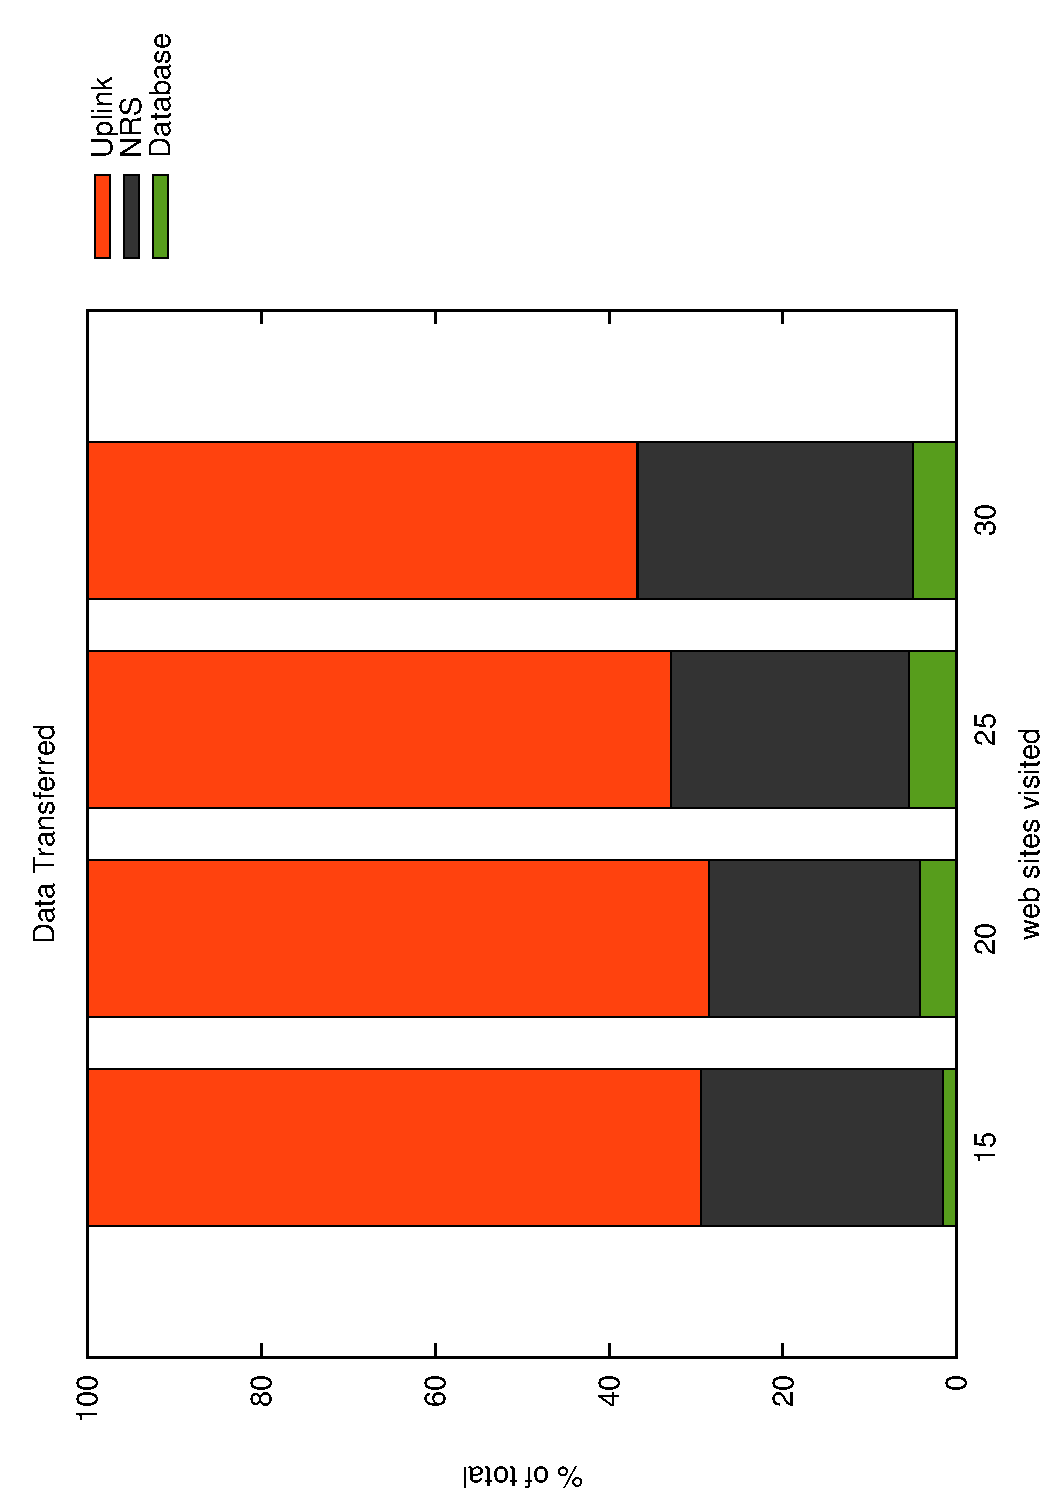
\includegraphics[width=0.62\textwidth, angle=-90]{./img/plots.pdf}
    	\caption{Results of Test 1}
	\label{fig:frontendtest1}
\end{figure}

\begin{figure}[H]
	\centering
		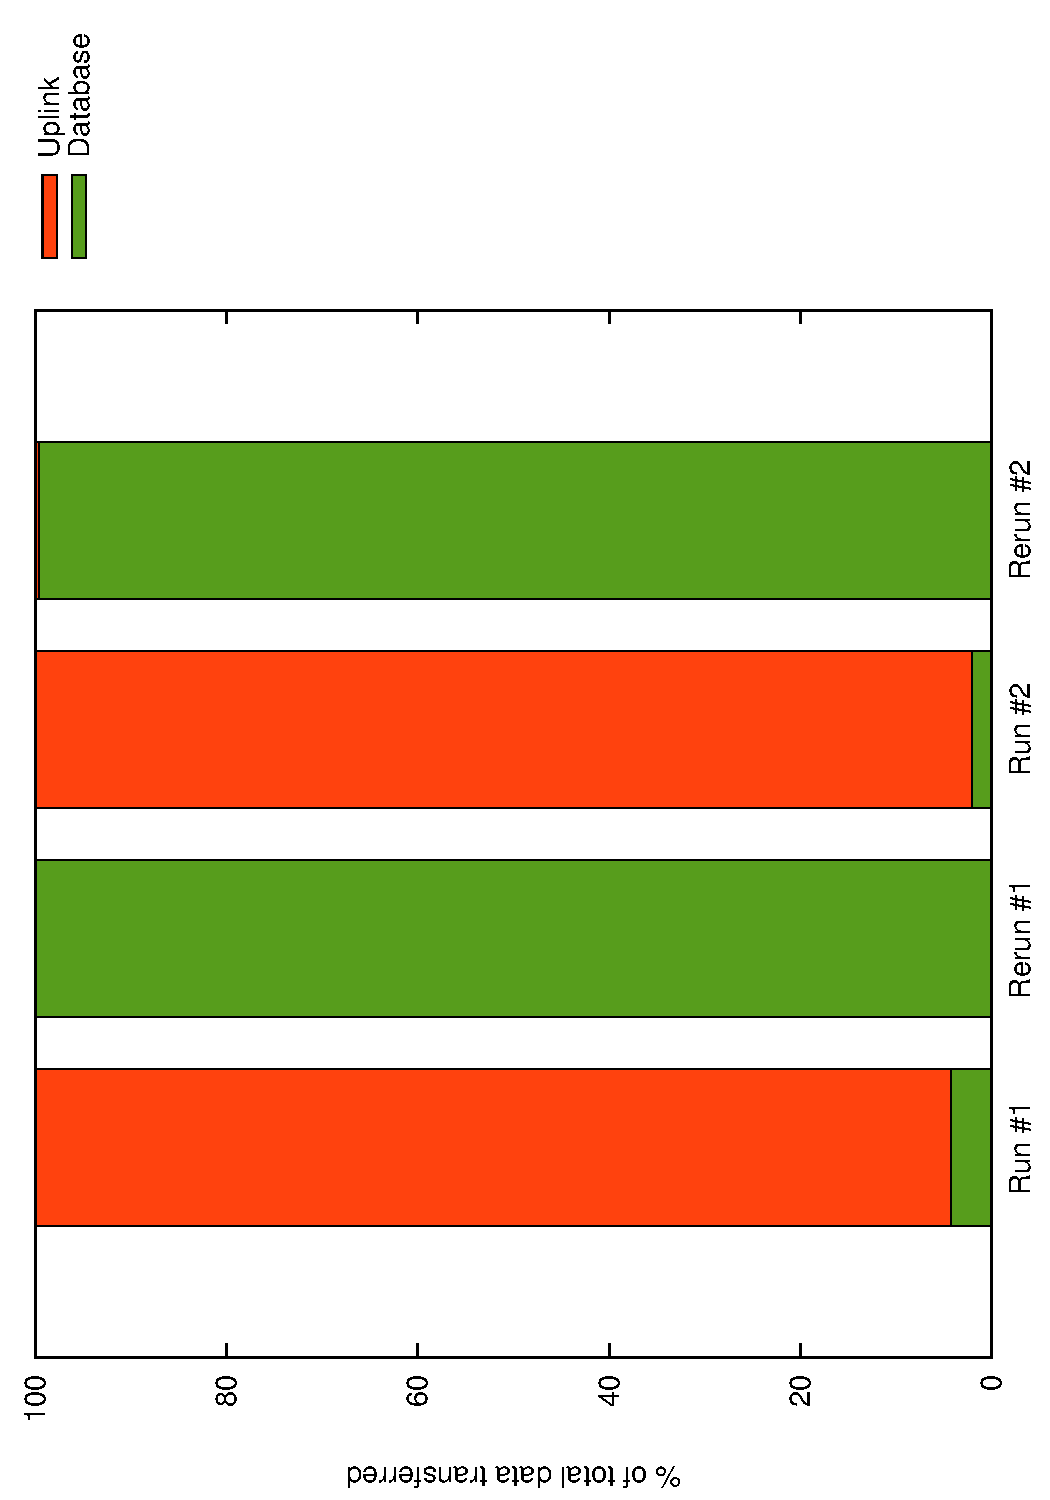
\includegraphics[width=0.62\textwidth, angle=-90]{./img/rerun.pdf}
    	\caption{Results of Test 2}
	\label{fig:frontendtest2}
\end{figure}

\begin{figure}[H]
	\centering
		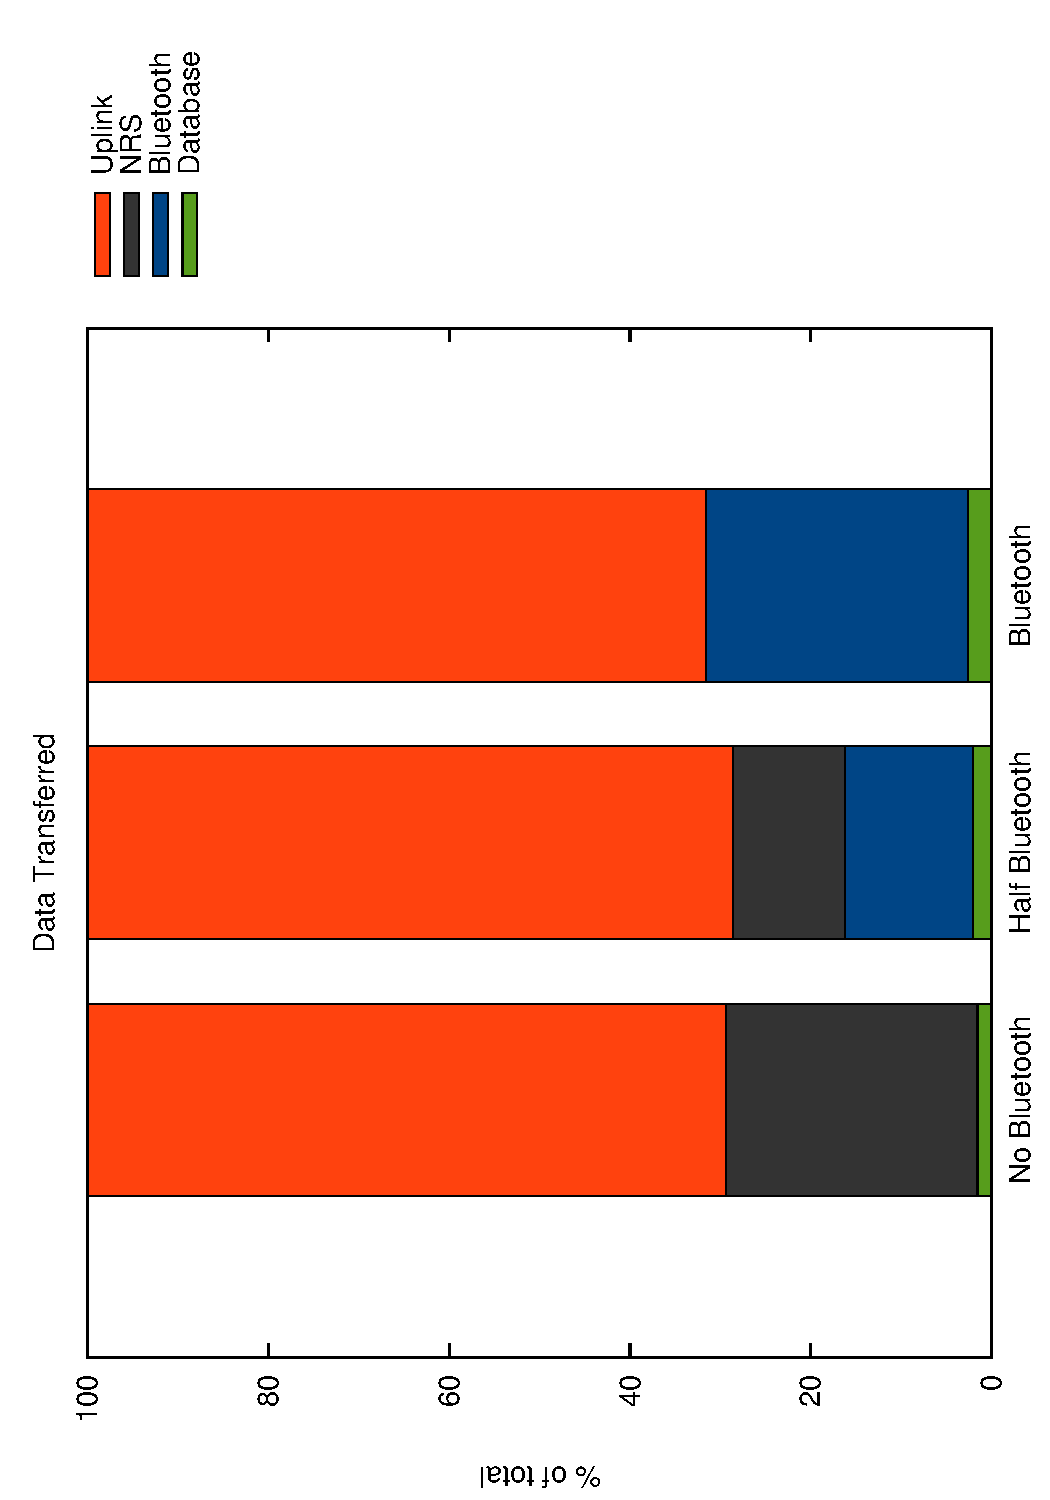
\includegraphics[width=0.62\textwidth, angle=-90]{./img/half_bt.pdf}
    	\caption{Results of Test 3}
	\label{fig:frontendtest3}
\end{figure}

\subsection{Discussion}

Figure \ref{fig:frontendtest1} shows that even without precaching, approximately 30\% of the data 
can be retrieved without accessing the Internet. With precaching of popular web pages this percentage could 
possibly increase even further.

It was observed that if one phone had a jump start on another phone to start retrieving a certain web page, 
the second phone shortly caught up with the first phone. The two phones then try to retrieve the same resource 
at the same time which will not be in the cache and both will use the Internet connection.

Furthermore it becomes apparent that a few percent of resources are retrieved from the 
database. This is because these resources are linked to several times throughout all web pages. 
Since the resource is cached in the database the first time, additional requests can use the database.

Figure \ref{fig:frontendtest2} demonstrates that when accessing a web page a second time, a small part still has to be 
retrieved using the Internet. An example of when this can happen is when a web page links to a resource using JavaScript 
to add a timestamp to the resource's URL. Because of the dynamic nature of this content, it will not be found in any cache when 
requested. Therefore, there will be a certain amount of resources that will have to be retrieved from the Internet repeatedly.

In Figure \ref{fig:frontendtest3} the amount of data retrieved without using the Internet is similar 
whether or not full put is used. This is as expected because the data that is not made available through full put should 
be available through Bluetooth. 

The retrieval of web pages using our Elephant browser is slow, as can be seen in Table \ref{tbl:times}.
According to the results, the actual transfer of files itself is not responsible for the
long run of retrieving a web page. The main culprit behind the long retrieval 
times seem to be the searches. When the application is running most of the time is spent 
searching. A search is done for every web resource and for every resolution service so that the time quickly adds up. 
Following, future work would be to investigate the bottleneck in our search and to improve the retrieval times of 
web pages in order to optimize Elephant. Of course, using this application in a real 
life situation right now probably only makes sense if there is no connection at all. 

One thing that is not immediately visible but effects the test result is the fact that the NetInfService randomly pauses in 
the background. If this happens, all publishe, get and search requests fail which in turn results in everything being 
retrieved from the Internet. It is suspected that this is caused by how the Android OS handles applications in the background.
